\chapter{Fit Model and Validation}

\begin{section}{Description of the Fit Model}
\label{sec:fit_model}

In order to determine the values of the background normalizations and nuisance parameters, as well as extract any signal that may be present, a maximum-likelihood fit to the observed data is performed. 
The full likelihood model can be written as the multiplication of a likelihood constructed from only the $\Nleps = 1$ bins and a likelihood constructed from only the $\Nleps = 0$ bins:
\begin{align}
\mathcal{L} = \mathcal{L}_{\Nleps = 1} \mathcal{L}_{\Nleps = 0}
\end{align}
where
\begin{align}
\mathcal{L}_{\Nleps = 1}& = \prod_{\substack{i\in\Njets\\ j\in\MJ\\ k \in\Nb}}
P(N_{ijk}|\mu^{\signal}\nu^{\signal}_{ijk} + \mu^{\ttbar}_{i}\nu^{\ttbar}_{ijk} + \mu^{\QCD}_{i}\nu^{\QCD}_{ijk} + \mu^{\Wjets}\nu^{\Wjets}_{ijk} + \nu^{\Other}_{ijk}) \nonumber \\
                        &\prod_{l\in\text{\ttbar norm.}} P(N_{ijk}|\theta_{l}) \prod_{l^{'}\!\in\text{QCD norm.}} P(N_{ijk}|\theta_{l^{'}}) \prod_{l^{''}\!\in\text{W+jets norm.}} P(N_{ijk}|\theta_{l^{''}}) \prod_{m\in\text{shape}} P(N_{ijk}|\theta_{m}),
\end{align}
and 
\begin{align}
\mathcal{L}_{\Nleps = 0} &= \prod_{\substack{i\in\Njets\\ j\in\MJ\\ i'\!= i + 1}}
P(N_{i'\!j}|\mu^{\signal}\nu^{\signal}_{i'\!j} + \mu^{\ttbar}_{i'}\nu^{\ttbar}_{i'\!j} + \mu^{\QCD}_{i'}\nu^{\QCD}_{i'\!j} + \nu^{\Wjets}_{i'\!j} + \nu^{\Other}_{i'\!j}) \nonumber \\
                         &\prod_{l\in\text{\ttbar norm.}} P(N_{i'\!j}|\theta_{l}) \prod_{l'\!\in\text{QCD norm.}} P(N_{i'\!j}|\theta_{l'}) \prod_{m\in\text{shape}} P(N_{i'\!j}|\theta_{m}).
\end{align}
Here, the indices $i$, $j$, and $k$ respectively run over the appropriate \Njets, \MJ, and \Nb bins of the analysis.
The value of $N_{ijk}$ is the data yield in the corresponding bin, the $\mu$ factors correspond to unconstrained normalization parameters, the $\nu$ factors are the simulated yields, and the $\theta$ factors represent nuisance parameters.
The sets of nuisance parameters ``\ttbar norm.''\ and ``\QCD norm.''\ correspond to the \MJ-connection normalization parameters discussed in Subsection~\ref{subsec:mj_connection}, while the nuisance parameter set ``\Wjets norm.''\ corresponds to the normalization parameters described in Section~\ref{sec:wjets_normalization}. 
The ``shape'' nuisance parameter set is comprised of those described in Chapter~\ref{chap:systematics}.
For conciseness, the dependencies of the $\nu$ terms and elements of the $\theta$ terms have been dropped but are kept for the discussion below.

In more detail, for the $\Nleps = 1$ likelihood, the $\mu^{\signal}\nu^{\signal}_{ijk}(\theta_m)$ term represents the signal yield in the corresponding bin, as a function of $\theta_m$, multiplied by a global signal strength parameter.
The $\mu^{\ttbar}_{i}\nu^{\ttbar}_{ijk}(\theta_m, \theta_{l,ij})$ term encodes the floating normalizations in each \Njets bin through $\mu^{\ttbar}_{i}$, while the effects of shape systematics and the \MJ-connection normalizations are represented by the dependence of $\nu^{\ttbar}_{ijk}$ on $\theta_m$ and $\theta_{l,ij}$, respectively.
The QCD term behaves analagously to the \ttbar term, except that it has separate \MJ-connection normalizations and, thus, is dependent on $\theta_{l'\!,ij}$ instead of $\theta_{l,ij}$.
The $\mu^{\Wjets}\nu^{\Wjets}_{ijk}(\theta_m, \theta_{l^{''}\!\!,i})$ term controls the \Wjets yield in the corresponding bin, which is dependent on an overall unconstrained normalization parameter, $\mu^{\Wjets}$, on shape systematics, $\theta_m$, and on \Njets-dependent normalizations, $\theta_{l^{''}\!\!,i}$.
Finally, the term $\nu^{\Other}_{ijk}(\theta_m)$ does not have a corresponding $\mu$ factor as the normalization of Other is taken from simulation.
The dependence on $\theta_m$, however, does allow the normalization to vary according to systematic uncertainties.

The $\Nleps = 0$ likelihood largely follows the same structure as the $\Nleps = 1$ likelihood, though with some important differences and features.
First, the data yields, $N_{i'\!j}$, and simulation yields, $\nu_{i'\!j}$, do not depend on the index $k$, reflecting the fact that the $\Nleps = 0$ regions are integrated in \Nb for $\Nb \geq 1$.
Second, the likelihood depends not on index $i$ but on $i'$, where $i' = i + 1$. This represents the correspondence of \Njets bins between the 0-lepton and 1-lepton regions, where a higher $\Njets$ bin in the $\Nleps = 0$ sample is used to constrain an \Njets bin in the $\Nleps = 1$ sample.
Third, the $\mu^{\ttbar}$ and $\mu^{\QCD}$ terms appear in this likelihood as well, indicating the simulataneous fit of their contributions across the two $\Nleps$ regions, while the $\mu^{\Wjets}$ term is not present, as the \Wjets normalization is only determined in the $\Nleps = 1$ region.
The \Wjets normalization is not simulataneously fit in both \Nleps regions, because it is negligibly small in the 0-lepton region.
This fact also explains why a product analagous to $\displaystyle \prod_{l^{''}\!\in\text{W+jets norm.}} P(N_{ijk}|\theta_{l^{''}})$ is not present.
Lastly, the product $\displaystyle \prod_{m\in\text{shape}} P(N_{i'\!j}|\theta_{m})$ only affects the term $\nu^{\Other}_{i'\!j}$, as for all other processes the shape variations have no effect due to the integration in \Nb.

\end{section}


\begin{section}{Validation of the Fit Model}

Due to the fit's complexity and many adjustable parameters, it is important to verify the fit model and that it behaves as intended.
Signal injection tests are simulation-based studies that allow for the assumptions of the model to be tested and, importantly, for the behavior of the fit in the presence of signal to be evaluated.
A control region fit is a data-driven validation test, which is needed to ensure that the method is not overly-reliant on simulation and is able to model the actual experimental conditions.
Both of these tests were performed to validate the fit model and are described in fuller detail below.

\end{section}

\begin{subsection}{Signal Injection Study}

Signal injection studies are a useful way to quantify how well the maximum-likelihood fit can extract a potential signal if it is indeed present.
These studies rely on the use of psuedodata experiments.
A single experiment consists of generating psuedodata by fluctuating bin yields around their pre-fit values according to their statistical and systematic uncertainties.
This pseudodata can then be treated as observations and can be fit with the results examined.
As many psuedodata experiments are generated, the collection of observations approximates the distribution of possible observations as defined by the fit model and as a result the distribution of post-fit results approximates the distribution of possible post-fit results.

For the signal injection study, 1000 experiments are generated by fluctuating both the expected background and signal yields (with signal strength = 1) for each gluino mass point.
Figure~\ref{fig:sig_injection} shows the median fitted signal strength of the 1000 experiments for each gluino mass point.
For gluino masses between $1000 - 1700~\GeV$ the fit shows no evidence of a bias and has a median extracted signal strength of $\sim$1, while for higher gluino masses, the fit tends to under-extract the signal contribution (up to $\sim$25\% for $\mglu = 2000~\GeV$).
These biased mass points correspond to models where the number of signal events is very low.
For example, there are only 8.6 events expected for the $\mglu = 2000~\GeV$ model, summing over all analysis bins.
This low yield means that gaussian-approximations of the poisson-distributed bin yields used in the fit model are no longer appropriate, leading to the bias in the fit.

In order to test this hypothesis, additional signal injection studies, each consisting of 1000 experiments, are performed for the $\mglu = 2000~\GeV$ mass point, where the injected signal strengths are 1x, 3x, 5x, 10x the nominal cross section.
The resulting median extracted signal is 78\%, 92\%, 95\%, and 98\% of the injected signal, respectively.
These results support the hypothesis, as, with increasing signal strength, the gaussian-approximations become increasingly accurate, allowing for the fit to properly extract the signal contributions.
The distributions of the fractional fitted signal strength for these tests are shown in Figure~\ref{fig:siginj_bias_study}.

\begin{figure}[tbp!]
\centering
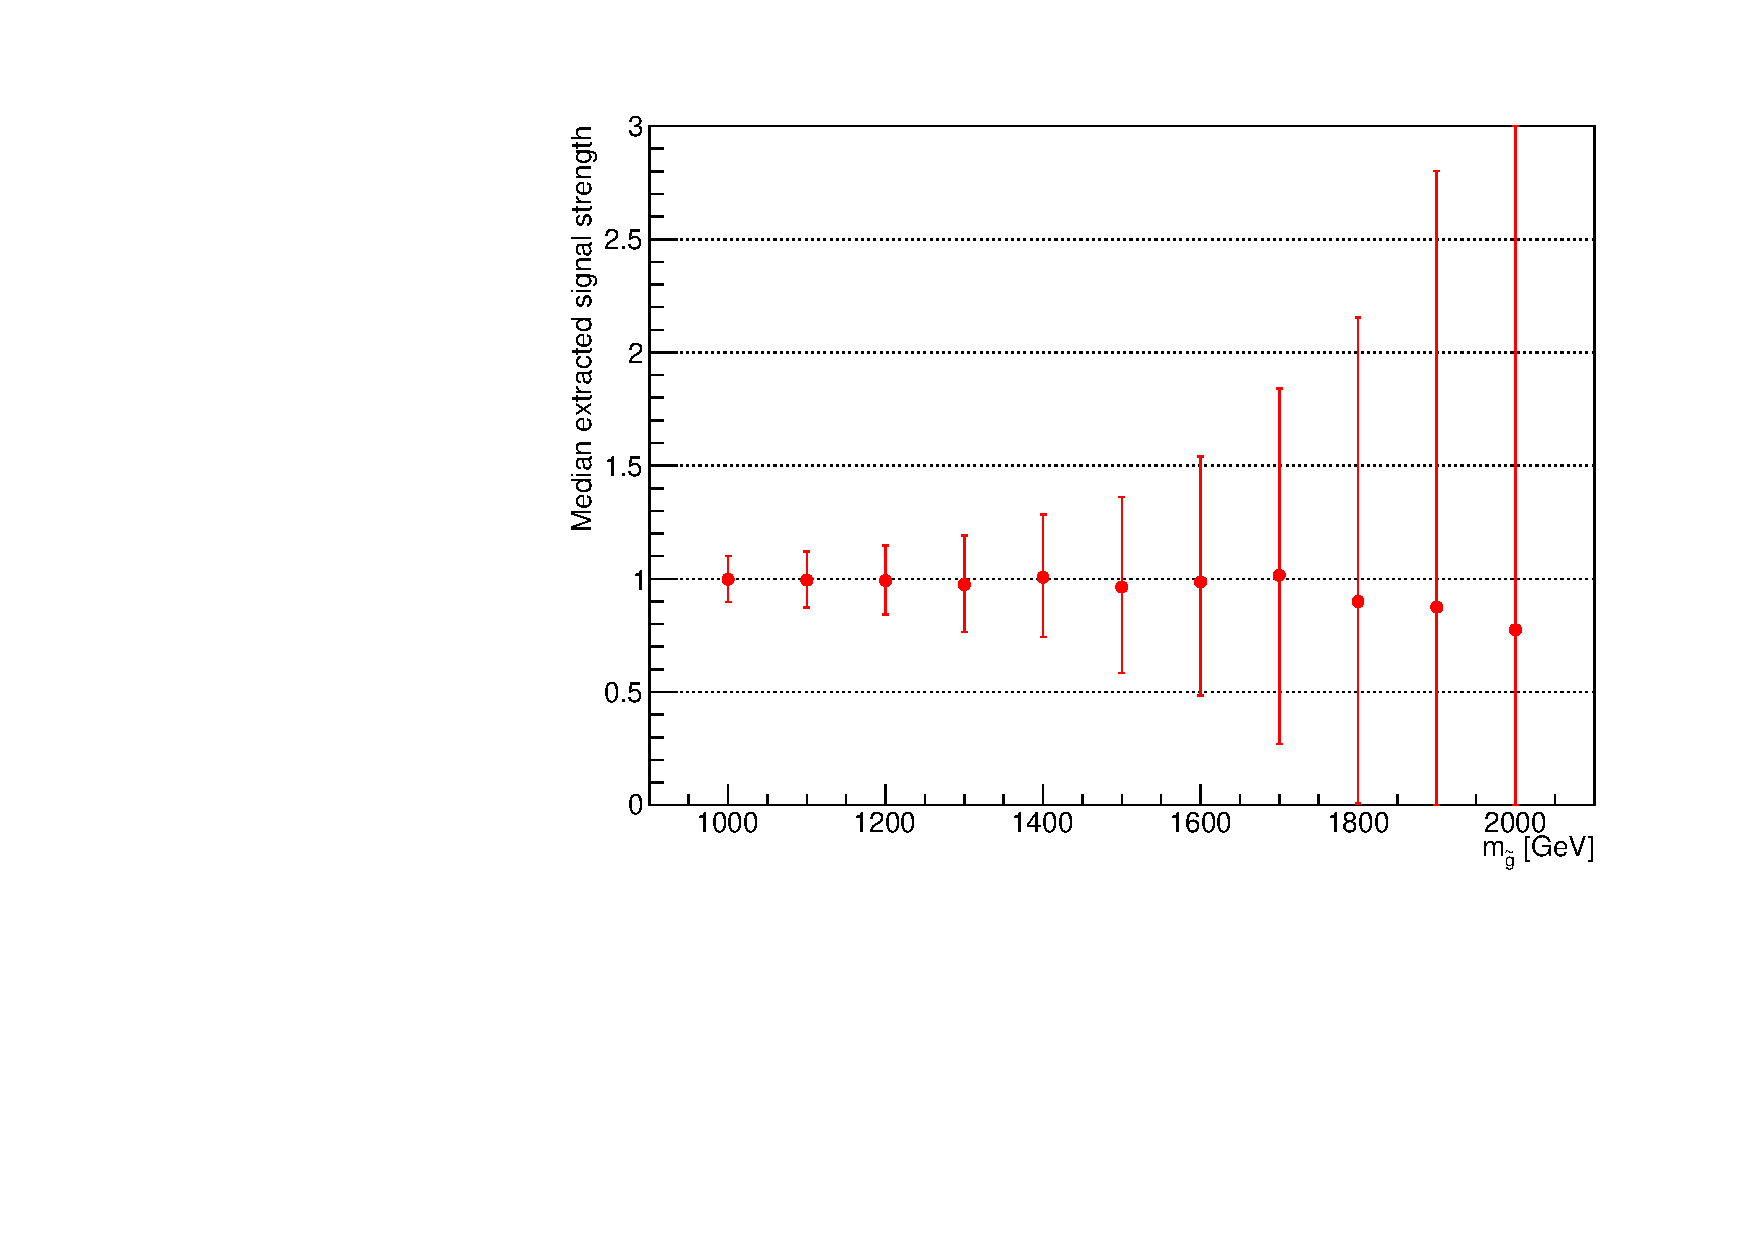
\includegraphics[angle=0,width=0.80\columnwidth]{fig/sig_injection.pdf}
\caption{Median extracted signal strength of 1000 psuedodata experiments as a function of gluino mass.
The uncertainties drawn are the median upper and lower errors of the fitted signal strengths per mass point.}
\label{fig:sig_injection}
\end{figure}

\begin{figure}[tbp!]
\centering
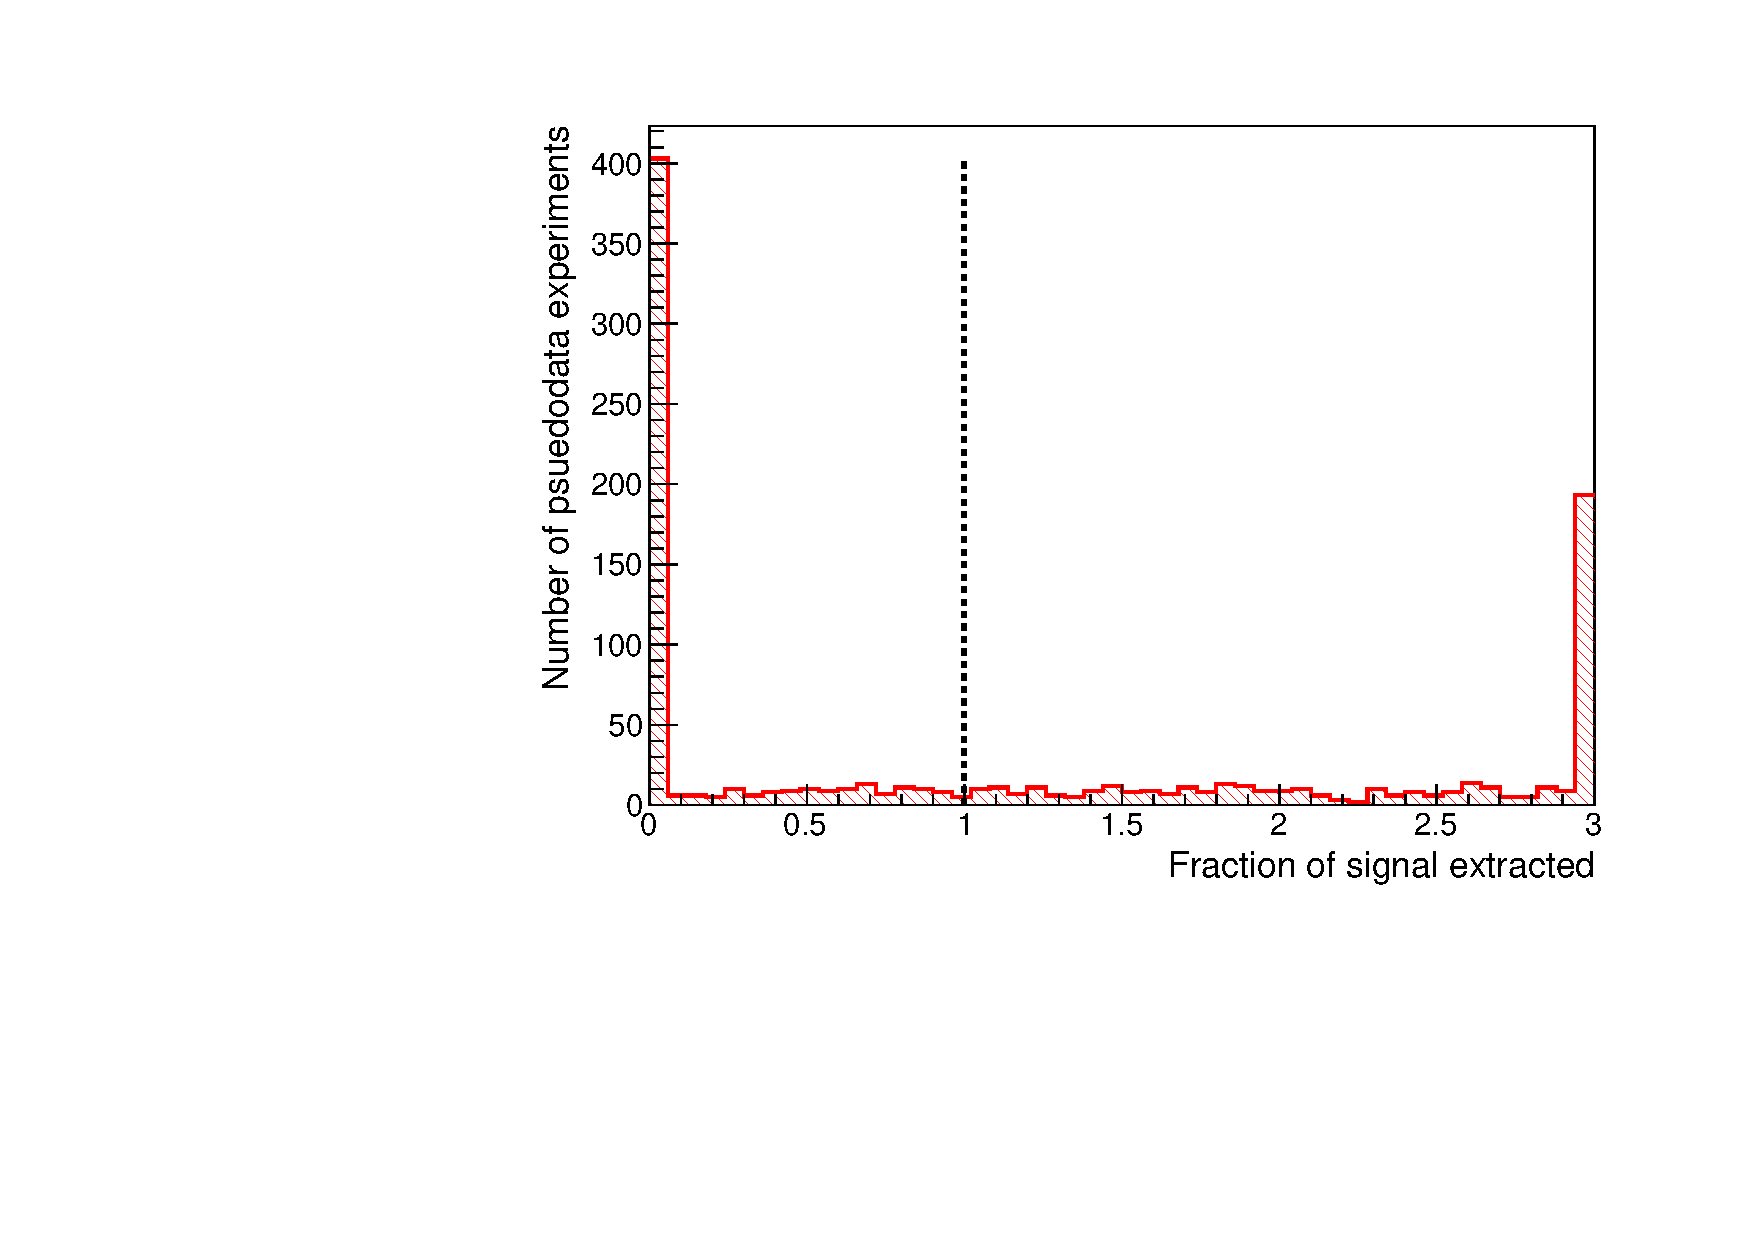
\includegraphics[angle=0,width=0.45\columnwidth]{fig/siginj_bias_1x.pdf}
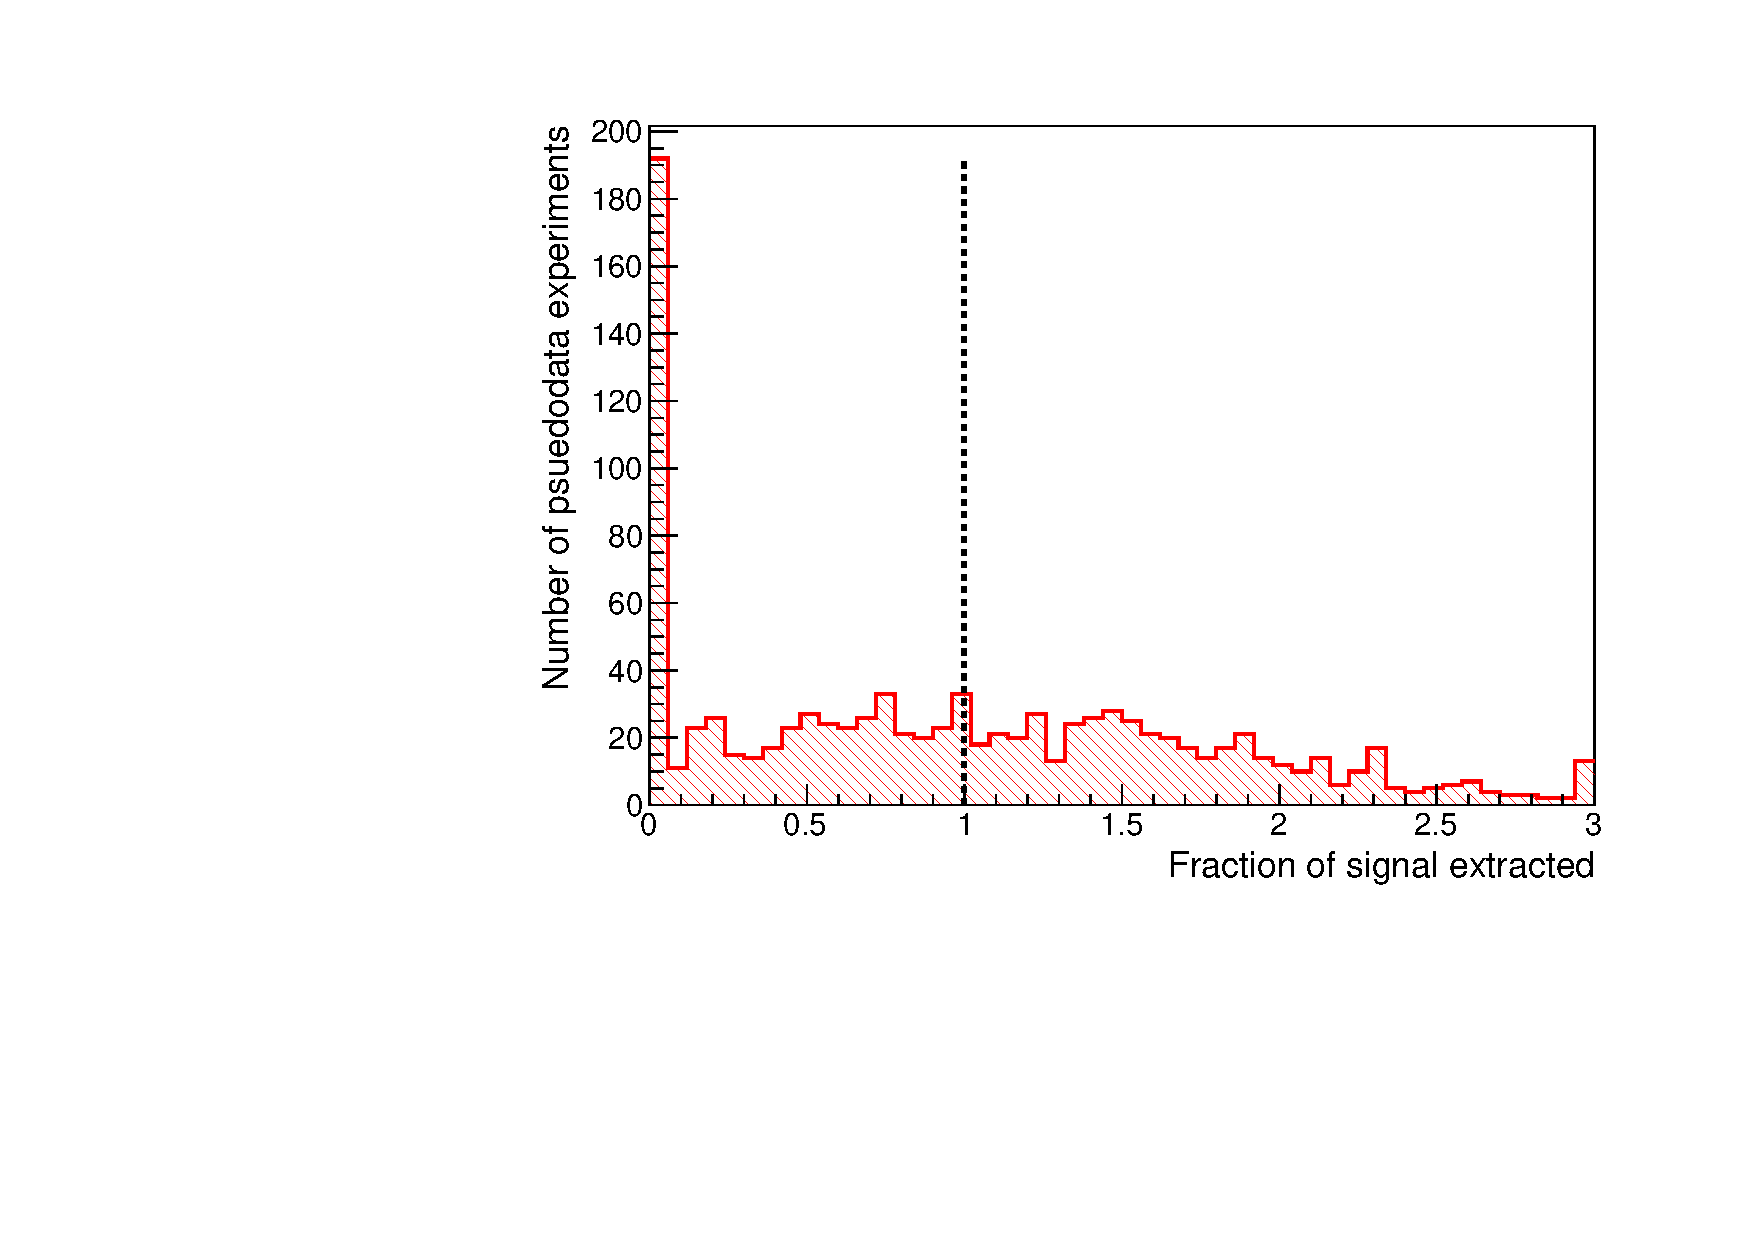
\includegraphics[angle=0,width=0.45\columnwidth]{fig/siginj_bias_3x.pdf}
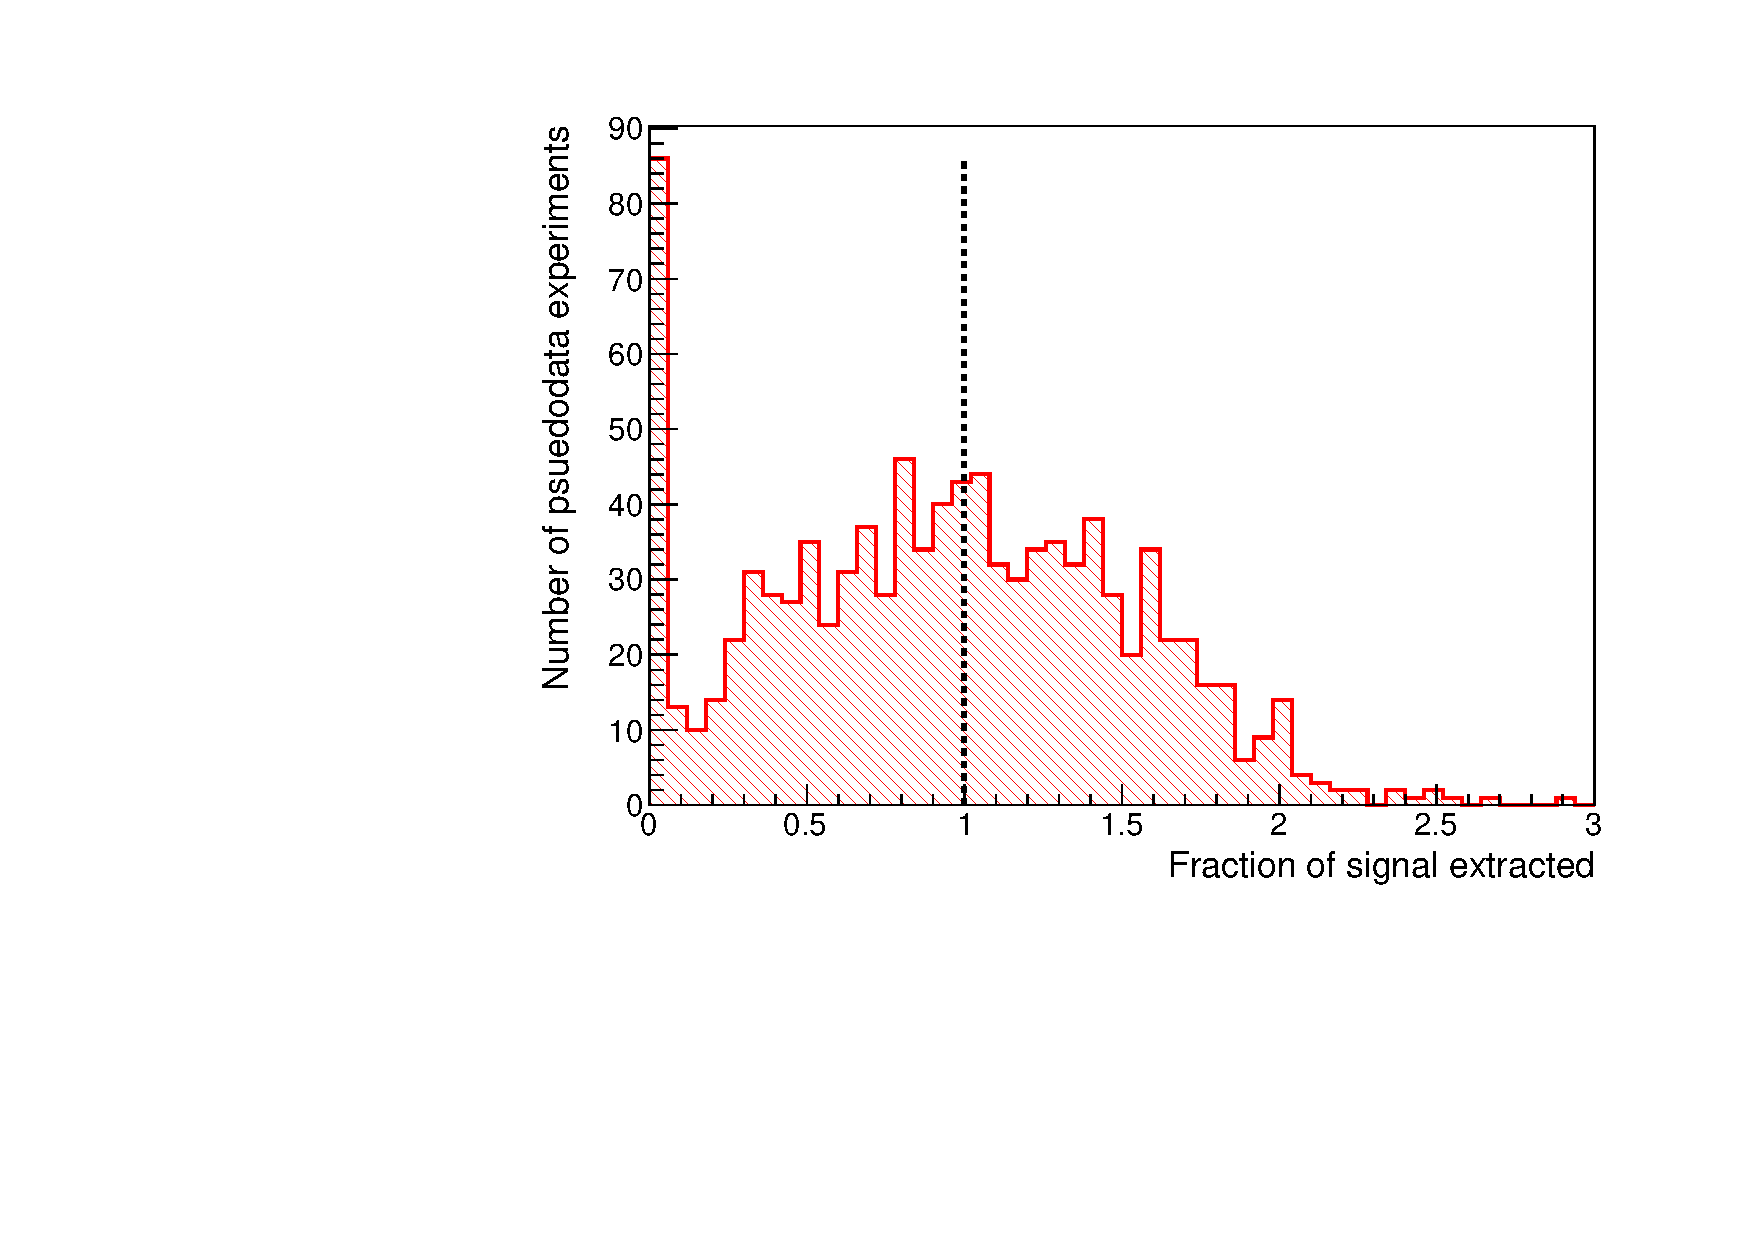
\includegraphics[angle=0,width=0.45\columnwidth]{fig/siginj_bias_5x.pdf}
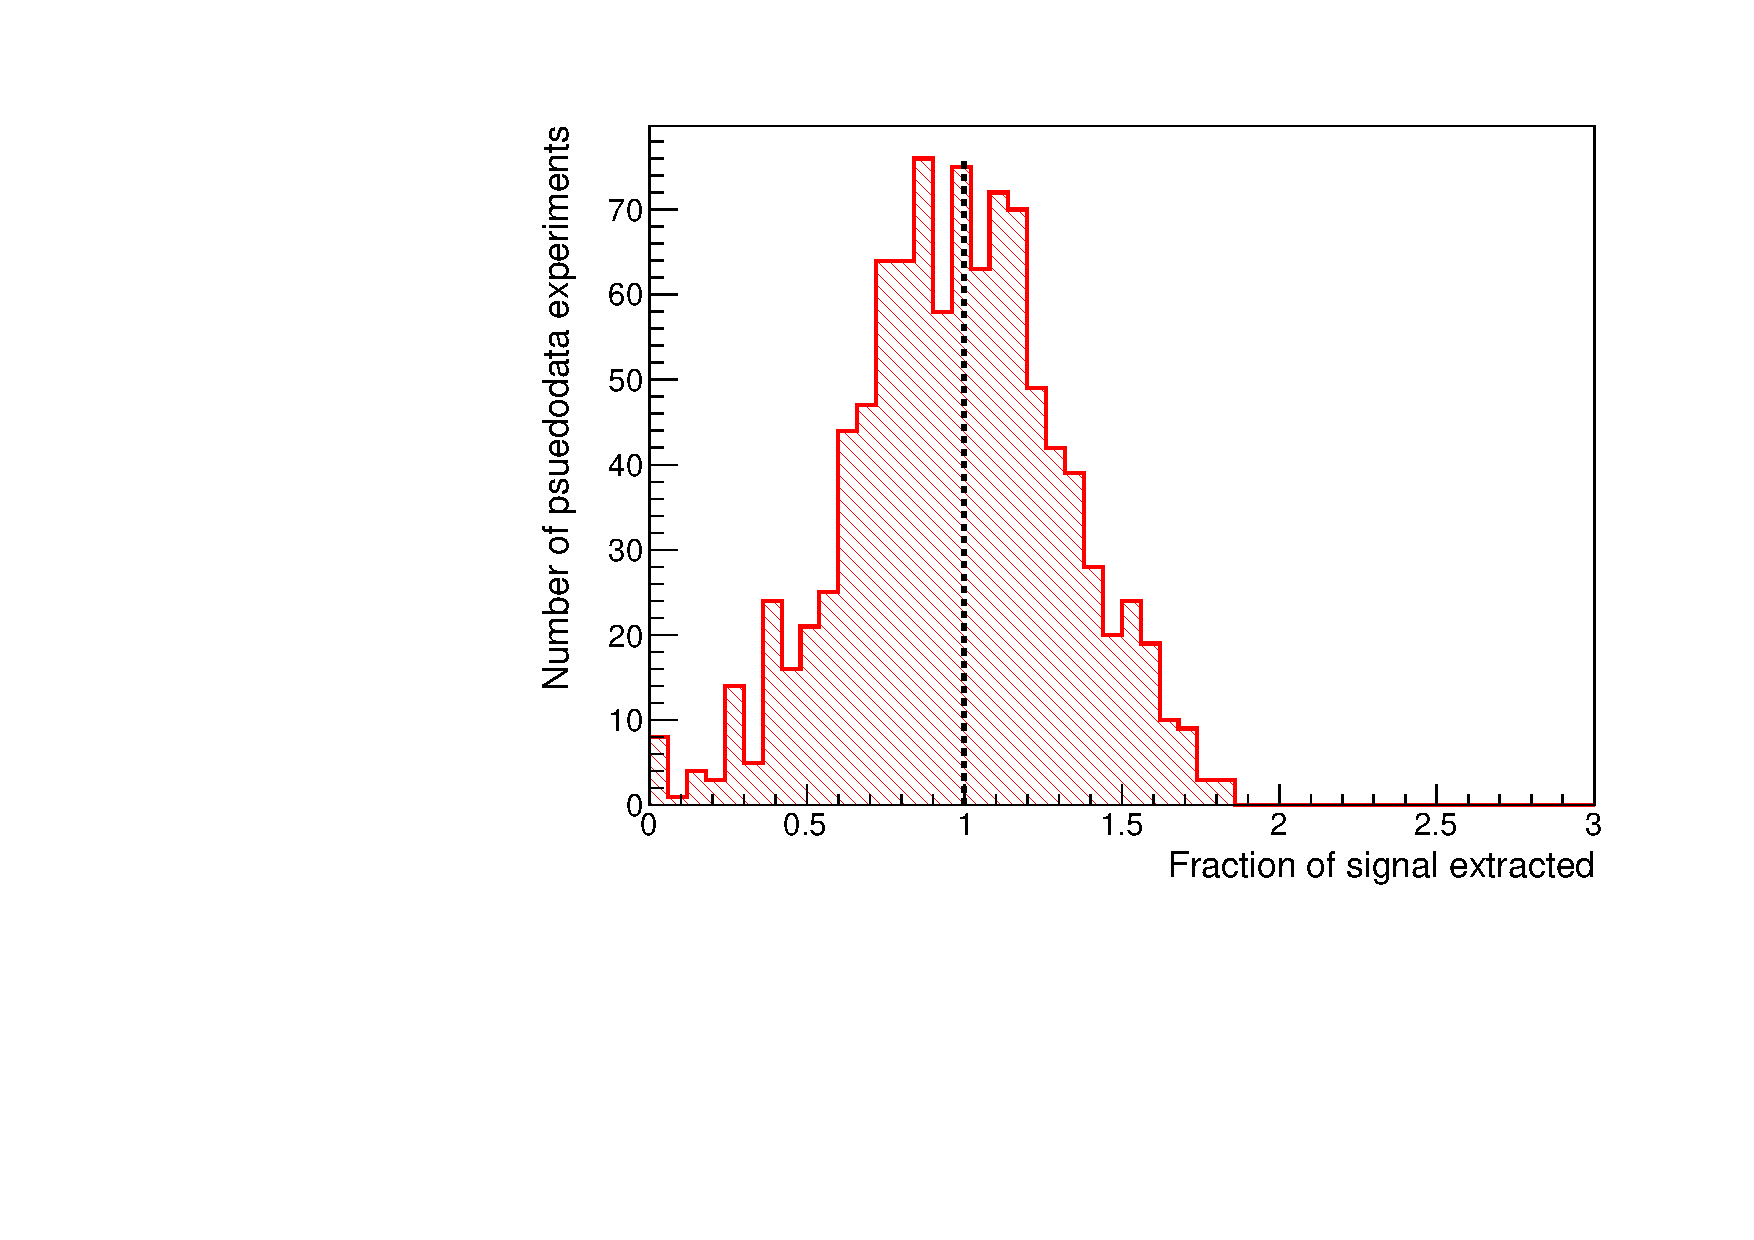
\includegraphics[angle=0,width=0.45\columnwidth]{fig/siginj_bias_10x.pdf}
\caption{Distribution of the fraction of signal extracted from 1000 psuedodata experiments for a 2000~\GeV gluino at 1x (top-left), 3x (top-right), 5x (bottom-left), and 10x (bottom-right) the nominal cross section.
The last bin includes the overflow contents, and the black dashed line represents extracting as much signal as was injected.
The median extracted signal is 78\%, 92\%, 95\%, and 98\% the injected signal, respectively.}
\label{fig:siginj_bias_study}
\end{figure}

No modifications to the fit model are made to correct for this issue.
This is because the fit bias only affects mass points that are far above the highest mass (1650~\GeV) expected to be excluded by this analysis, and Figure~\ref{fig:sig_injection} shows that the fit bias is much smaller than the precision of the fit for those mass points.
Additionally, the coverage of the 95\% confidence intervals of the fit is tested using the signal injection experiments and found to be either correct or slightly conservative, as shown in Table~\ref{tab:siginj_coverage}.

\begin{table}[tbp!]
\centering
\begin{tabular}{ |c|c|c| }
\hline
$\mglu = 1800~\GeV$ & $\mglu = 1900~\GeV$ & $\mglu = 2000~\GeV$ \\ \hline
$96\%$              & $95\%$              & $96\%$              \\ \hline
\end{tabular}
\caption{Actual coverage probability of the 95\% confidence interval of the fit for the mass points with a biased signal extraction.}
\label{tab:siginj_coverage}
\end{table}

\end{subsection}

\begin{subsection}{Control Region Fit}
\label{subsec:crfit}

While the signal injection studies are a useful validation of the fit model, it is important to validate the model using data in order to test for unmodeled effects.
This is done by performing the maximum-likelihood fit with only the low-\Njets, low-\MJ control regions, as defined in Table~\ref{fig:analysis_regions}.
These bins are chosen due to their low-expected signal yields, which avoids signal contamination effects and unblinding the high-expected signal regions in the case further modifications of the fit are required.

The control region fit, under the background-only hypothesis, is able to model the observed data well without needing large adjustments to the nuisance parameters, as seen in the post-fit \Nb distributions shown in Figure~\ref{fig:crfit}.
The change between the pre- and post-fit normalizations of the background processes is shown in Table~\ref{tab:crfit_norms}, while the pulls of the nuisance parameters corresponding to the systematic uncertainties (largely controlling the shape of the \Nb distribution) are shown in Figure~\ref{fig:crfit_pulls}.
Both sets of values are well-behaved, as the largest change in normalization is less than 50\% with typical values around 10-15\%, while the nuisance parameters are all consistent with their pre-fit uncertainties, with most shifted less than 0.05~s.d.
The largest pulls correspond to nuisance parameters controlling the gluon splitting rate (gs, +0.42~s.d.), the light-flavor b-tag SFs (btag\_udsg, +0.37~s.d.), and the heavy-flavor b-tag SFs (btag\_bc, +0.13~s.d.).
These nuisances are expected to be shifted up as the observed data is higher than simulation in the tail of the pre-fit \Nb distributions, as seen in Figure~\ref{fig:prefit_cr}, where the background simulation is normalized to match the observed data yields with a single scaling factor and with the pre-fit uncertainty represented by a hatched band.

\begin{figure}[tbp!]
\begin{center}
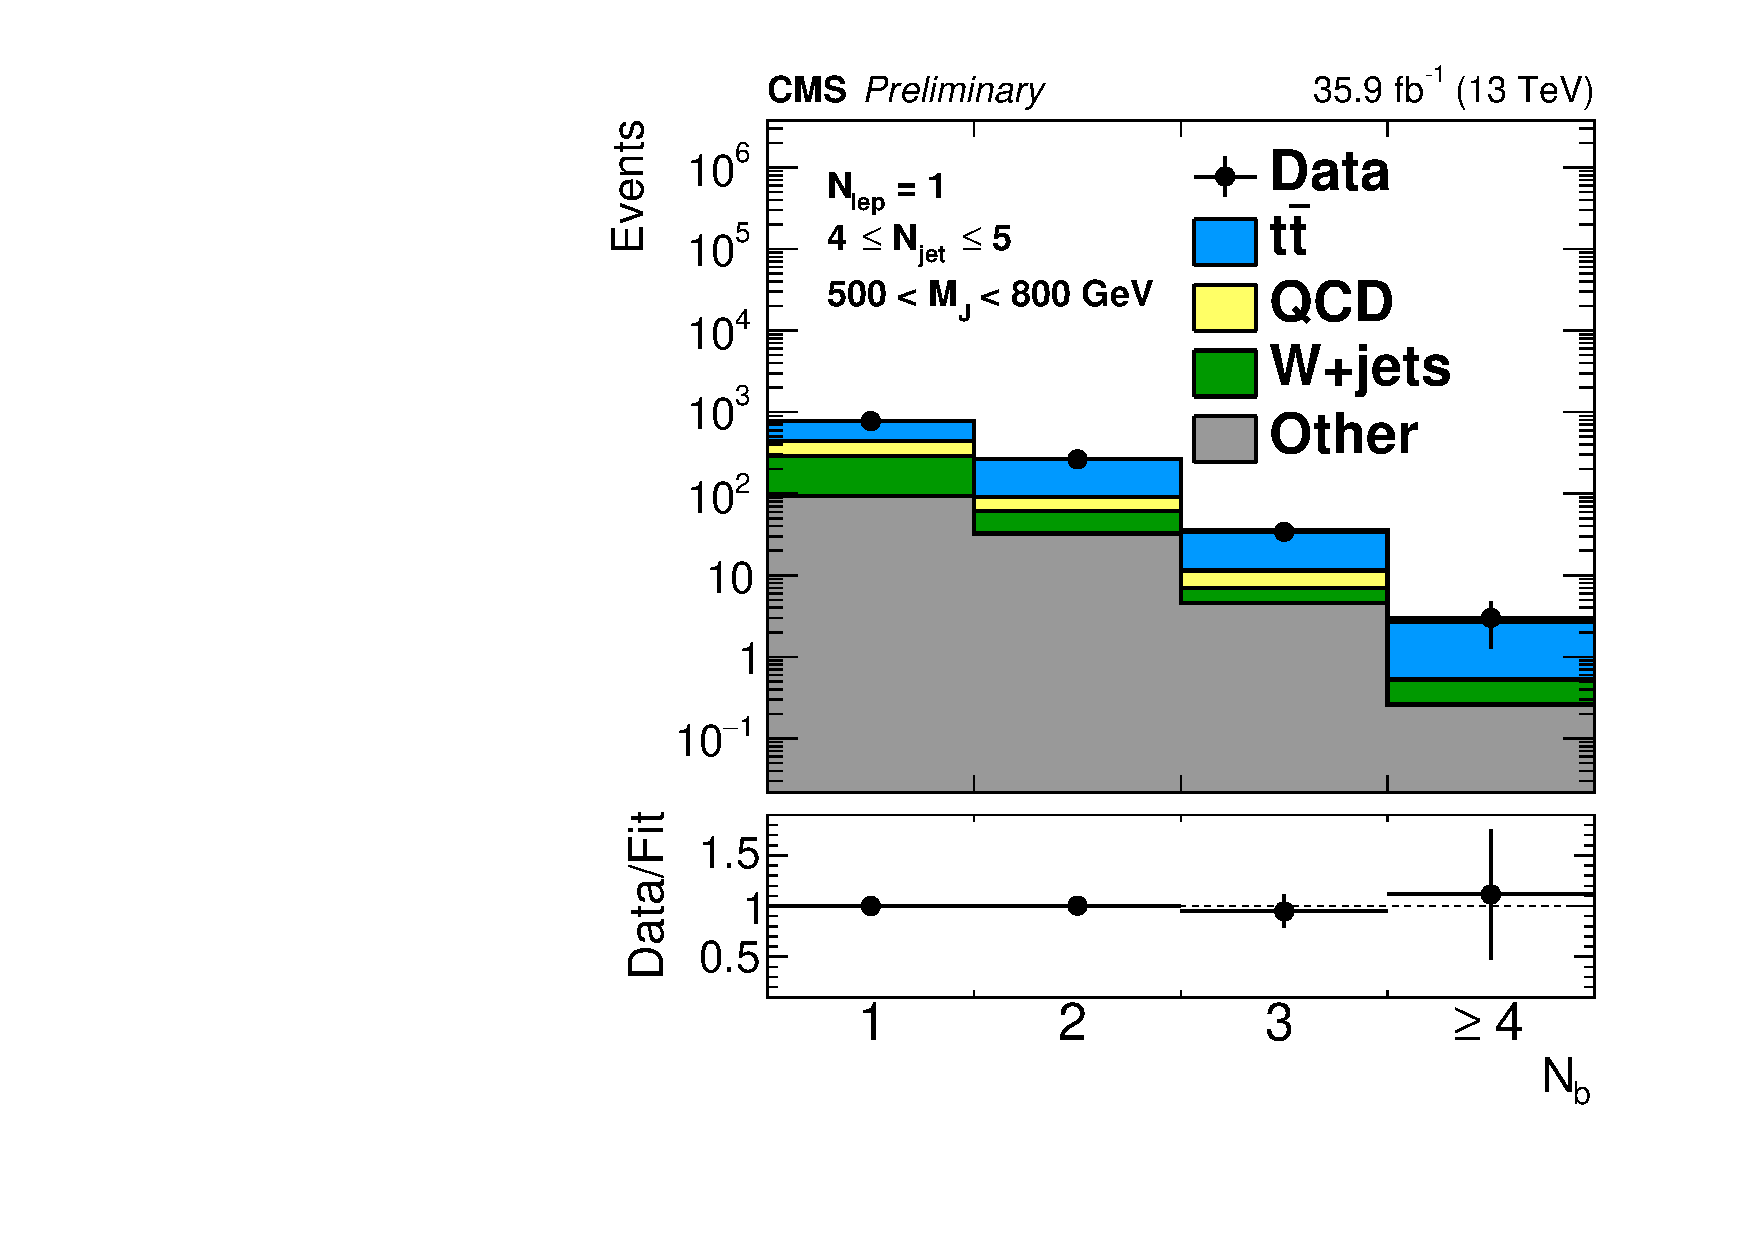
\includegraphics[angle=0,width=0.32\columnwidth]{fig/crfit_nlep1_nj45_lowmj.pdf}
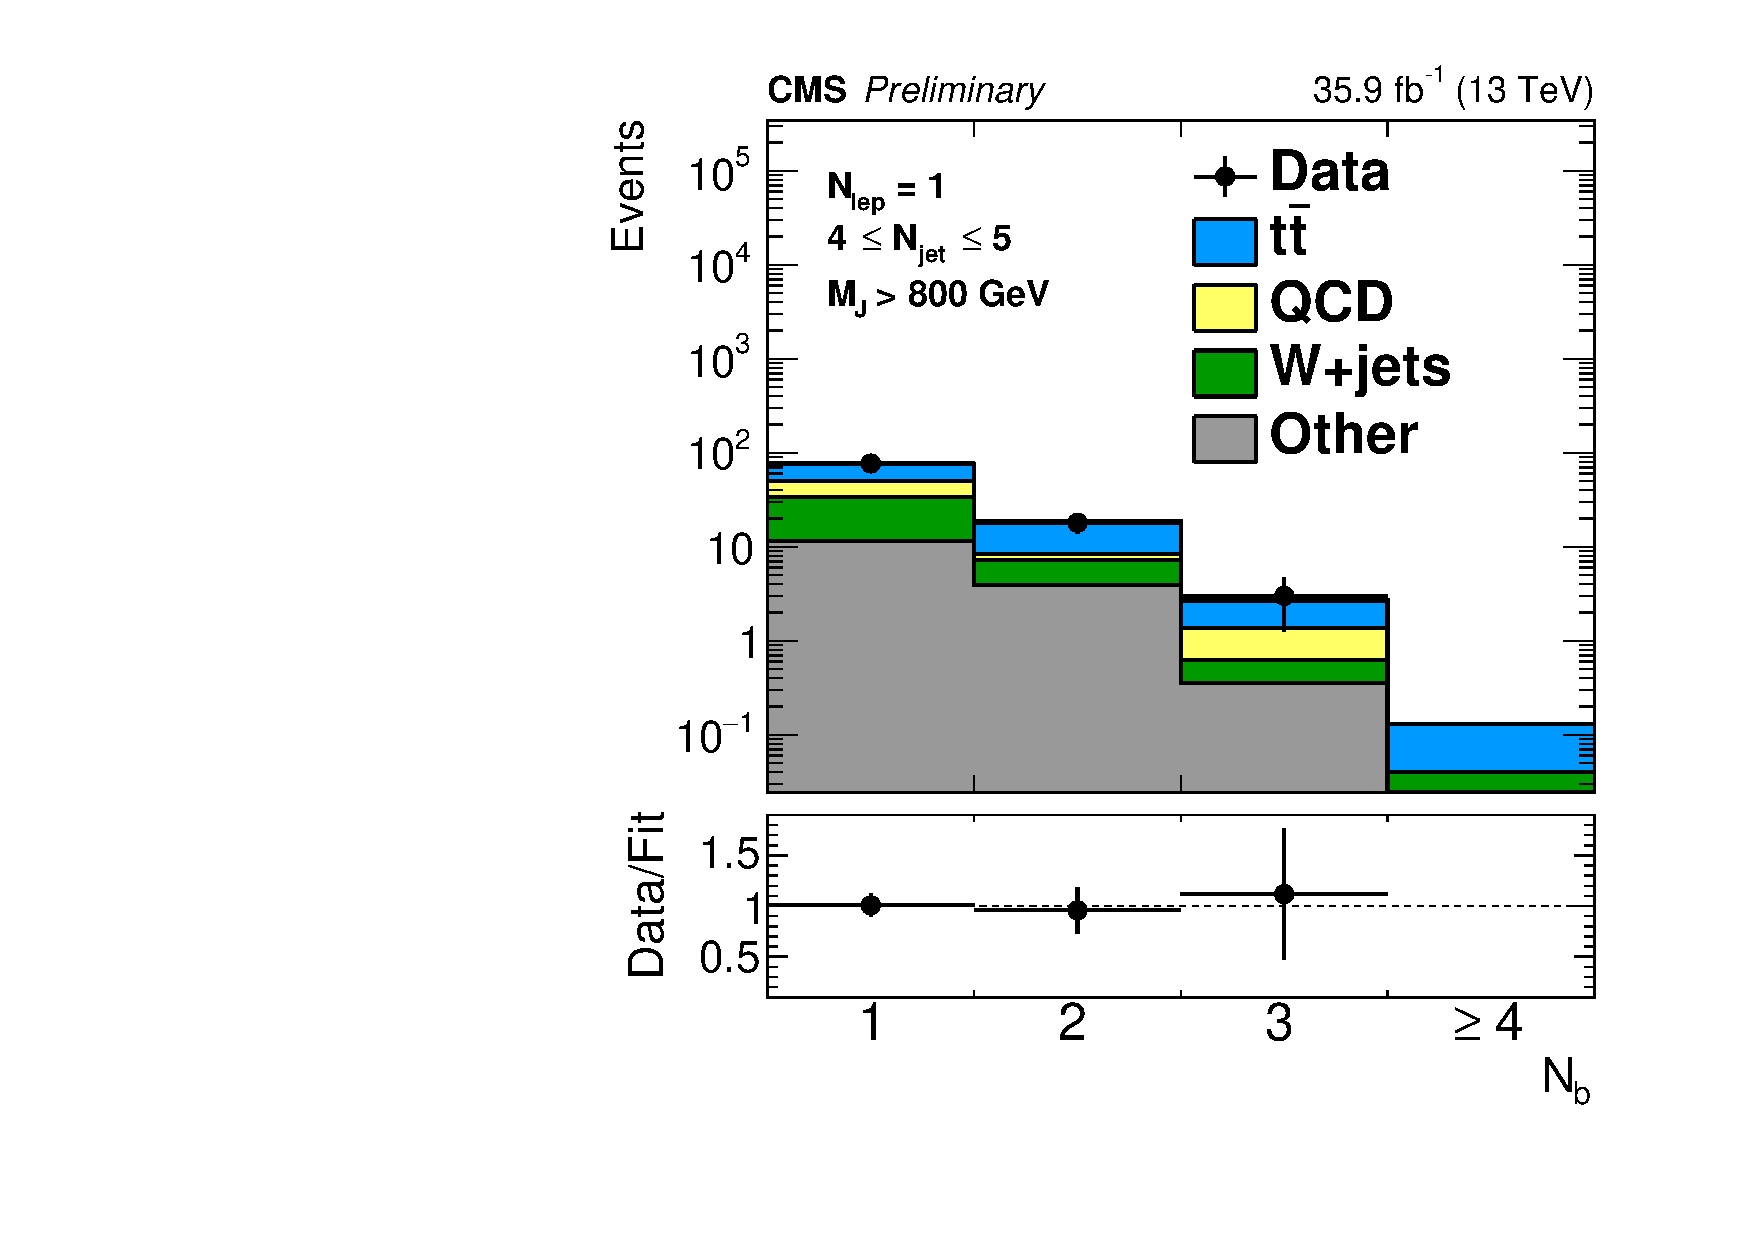
\includegraphics[angle=0,width=0.32\columnwidth]{fig/crfit_nlep1_nj45_highmj.pdf}
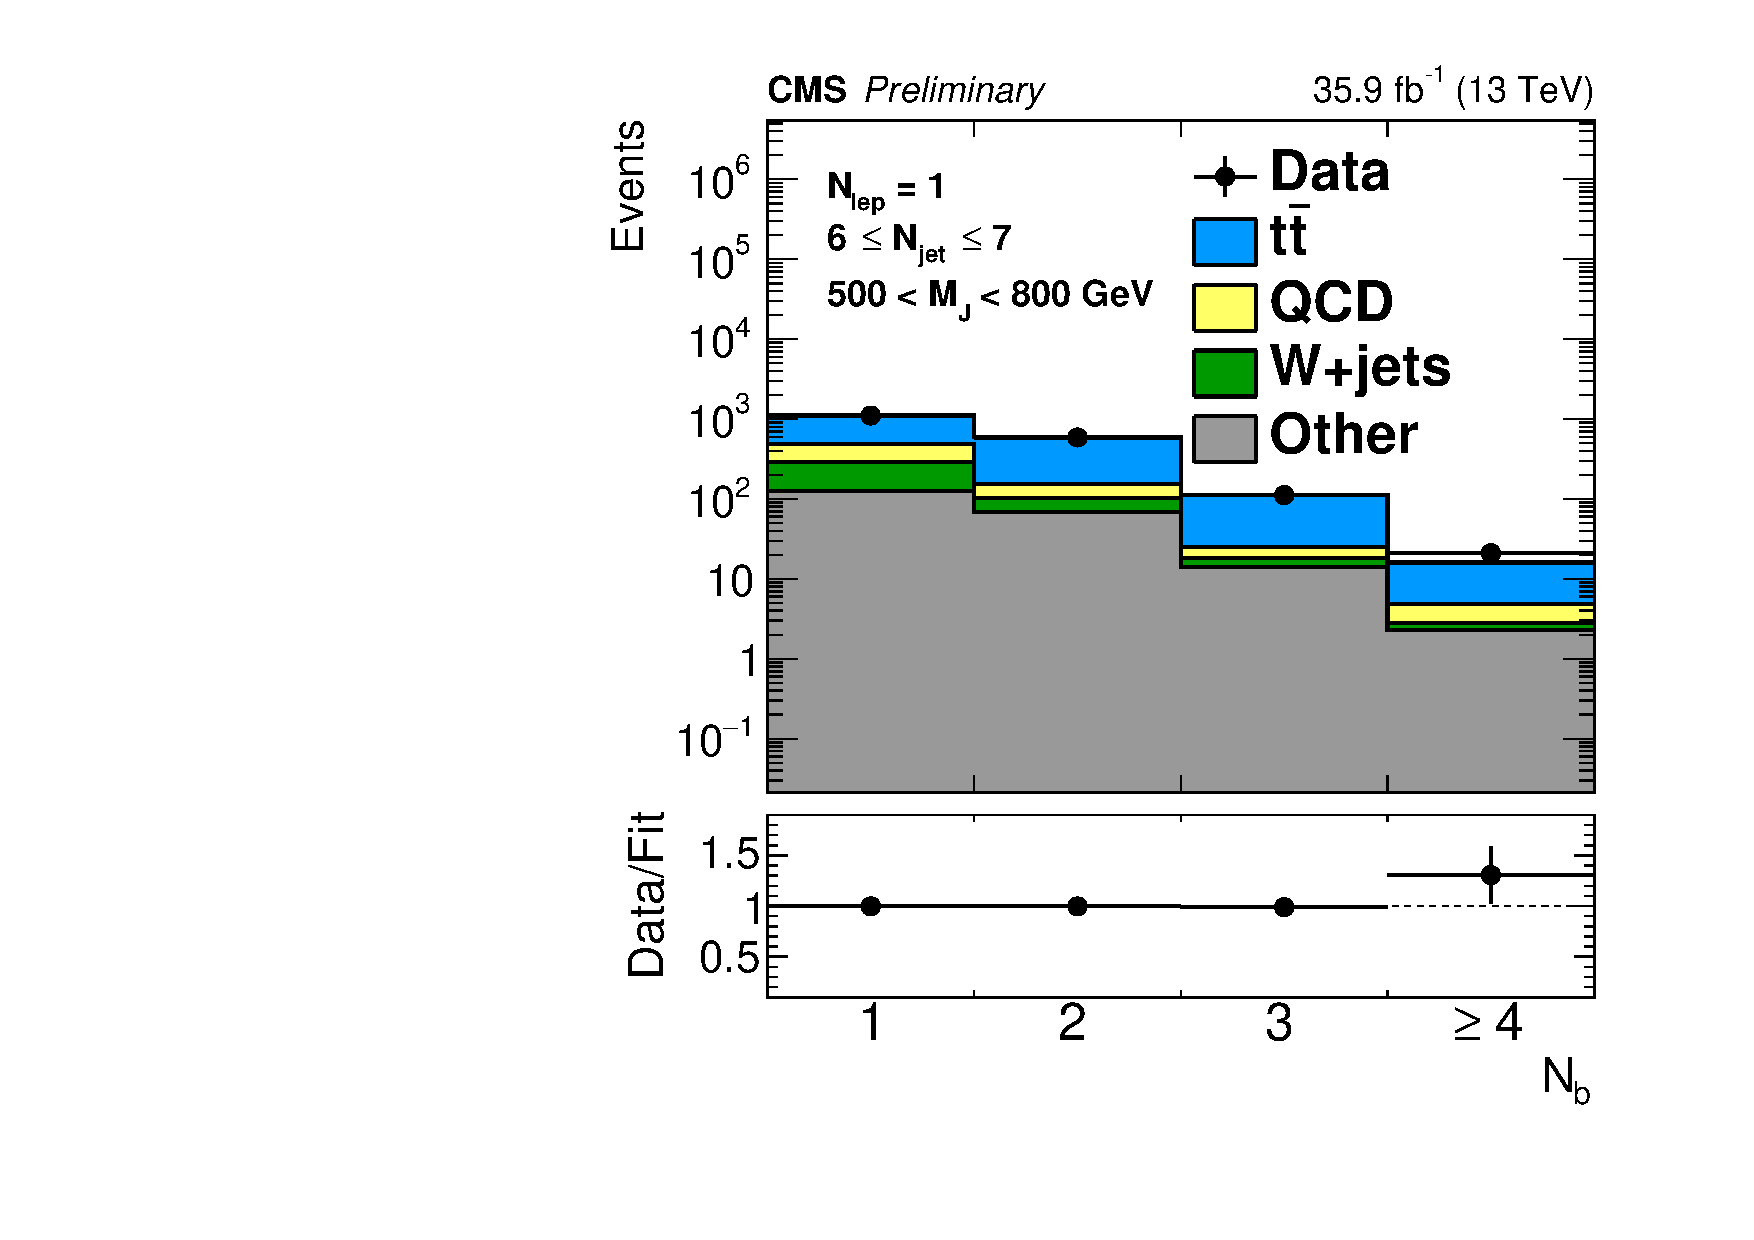
\includegraphics[angle=0,width=0.32\columnwidth]{fig/crfit_nlep1_nj67_lowmj.pdf}
\end{center}
\caption{Post-fit \Nb distributions of the control region fit with only statistical uncertainties shown.}
\label{fig:crfit}
\end{figure}

\begin{table}[tbp!]
\begin{center}
\begin{tabular}{|l|r|r|r|} \hline
Process   &   Pre-fit Yield   &  Post-fit Yield (b-only)   &   \% change \\
\hline
\hline
\multicolumn{4}{|c|}{$4 \leq \Njets \leq 5$, $500 \leq \MJ \leq 800$}         \\
\hline

\ttbar    &   501.4           &   $533.3  \pm  80.7$           &   +6.3      \\
QCD       &   218.8           &   $186.7  \pm  36.8$           &   -14.7     \\
\Wjets    &   400.4           &   $225.5  \pm  100.0$          &   -43.7     \\
Other     &   141.4           &   $131.8  \pm  34.5$           &   -6.8      \\

\hline
\multicolumn{4}{|c|}{$4 \leq \Njets \leq 5$, $\MJ \geq 800$}                 \\
\hline

\ttbar    &   36.9            &   $37.5   \pm  13.3$           &   +1.6      \\
QCD       &   23.1            &   $18.9   \pm  4.5$            &   -18.2     \\
\Wjets    &   45.7            &   $25.7   \pm  11.4$           &   -43.8     \\
Other     &   16.8            &   $15.7   \pm  3.8$            &   -6.5      \\

\hline
\multicolumn{4}{|c|}{$6 \leq \Njets \leq 7$, $500 \leq \MJ \leq 800$}        \\
\hline

\ttbar    &   1370.4          &   $1148.3 \pm  78.0$           &   -16.2     \\
QCD       &   293.9           &   $262.6  \pm  52.1$           &   -10.6     \\
\Wjets    &   367.7           &   $205.6  \pm  92.2$           &   -44.1     \\
Other     &   225.2           &   $209.7  \pm  58.5$           &   -6.9      \\
\hline
\end{tabular}
\caption{Table comparing the post-fit normalizations of the control region fit to the pre-fit yields for the various background processes.}
\label{tab:crfit_norms}
\end{center}
\end{table}


\begin{figure}[tbp!]
\begin{center}
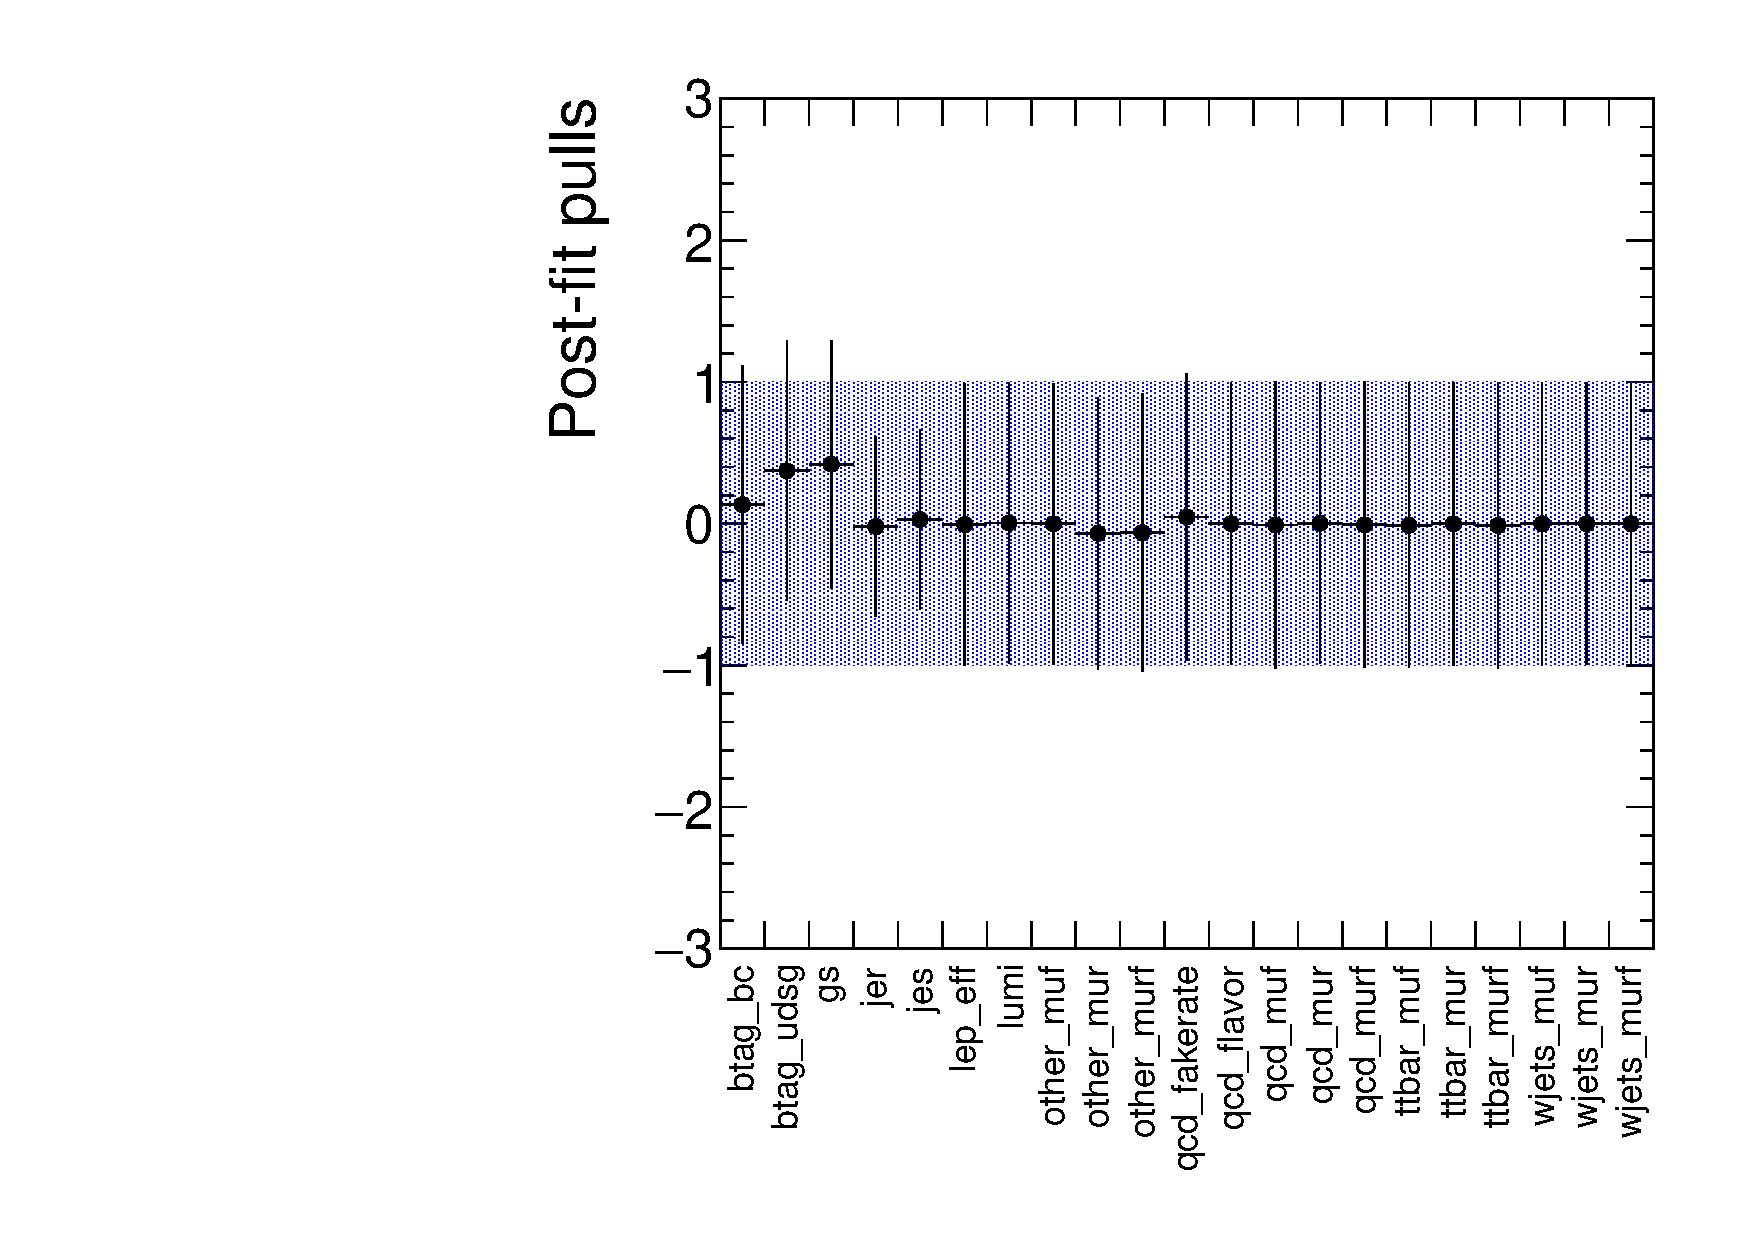
\includegraphics[angle=0,width=0.80\columnwidth]{fig/crfit_pulls.pdf}
\end{center}
\caption{Post-fit pulls of the background-only control region fit. 
The post-fit values of the nuisance parameters are indicated by data points, while the post-fit uncertainty is shown as a black line and is normalized by the pre-fit uncertainty depicted as the blue band.}
\label{fig:crfit_pulls}
\end{figure}

\begin{figure}[tbp!]
\begin{center}
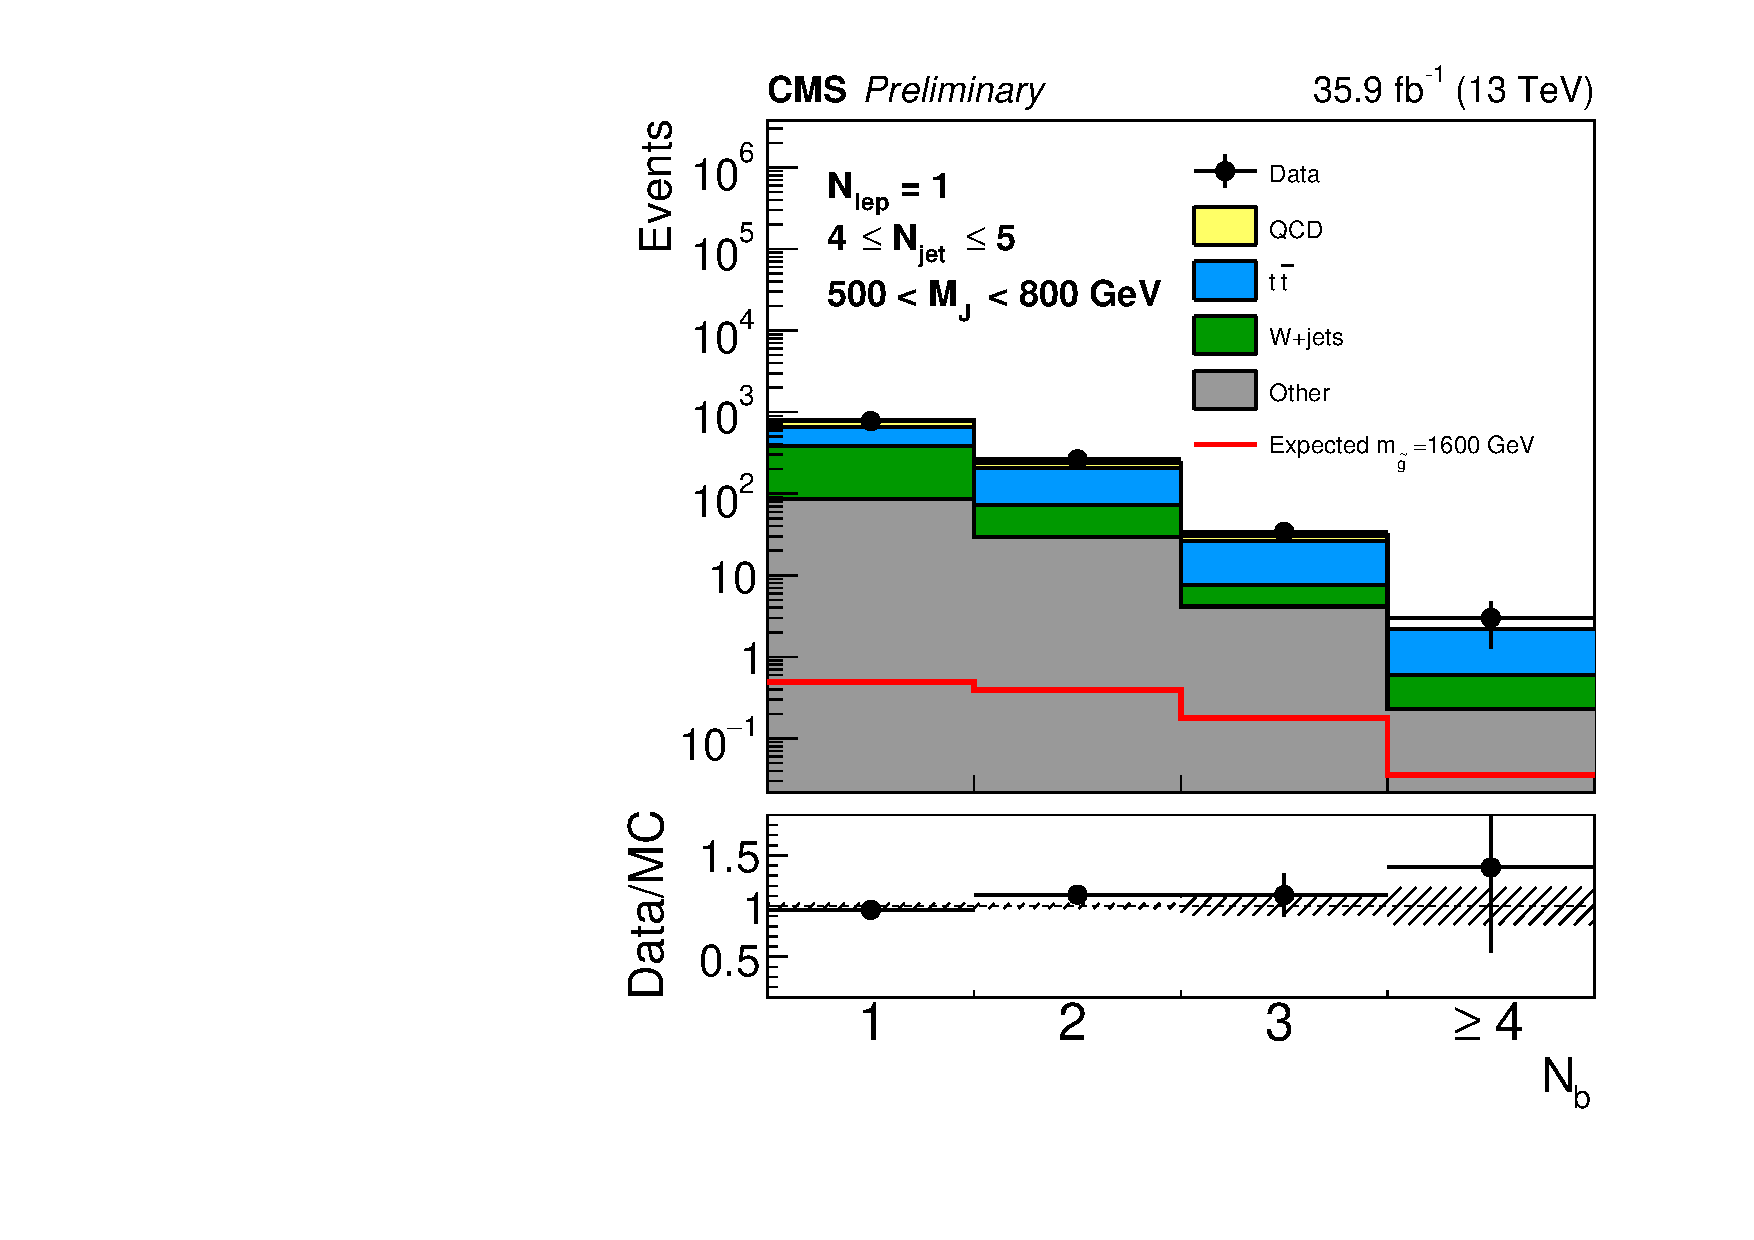
\includegraphics[angle=0,width=0.32\columnwidth]{fig/prefit_nlep1_nj45_lowmj.pdf}
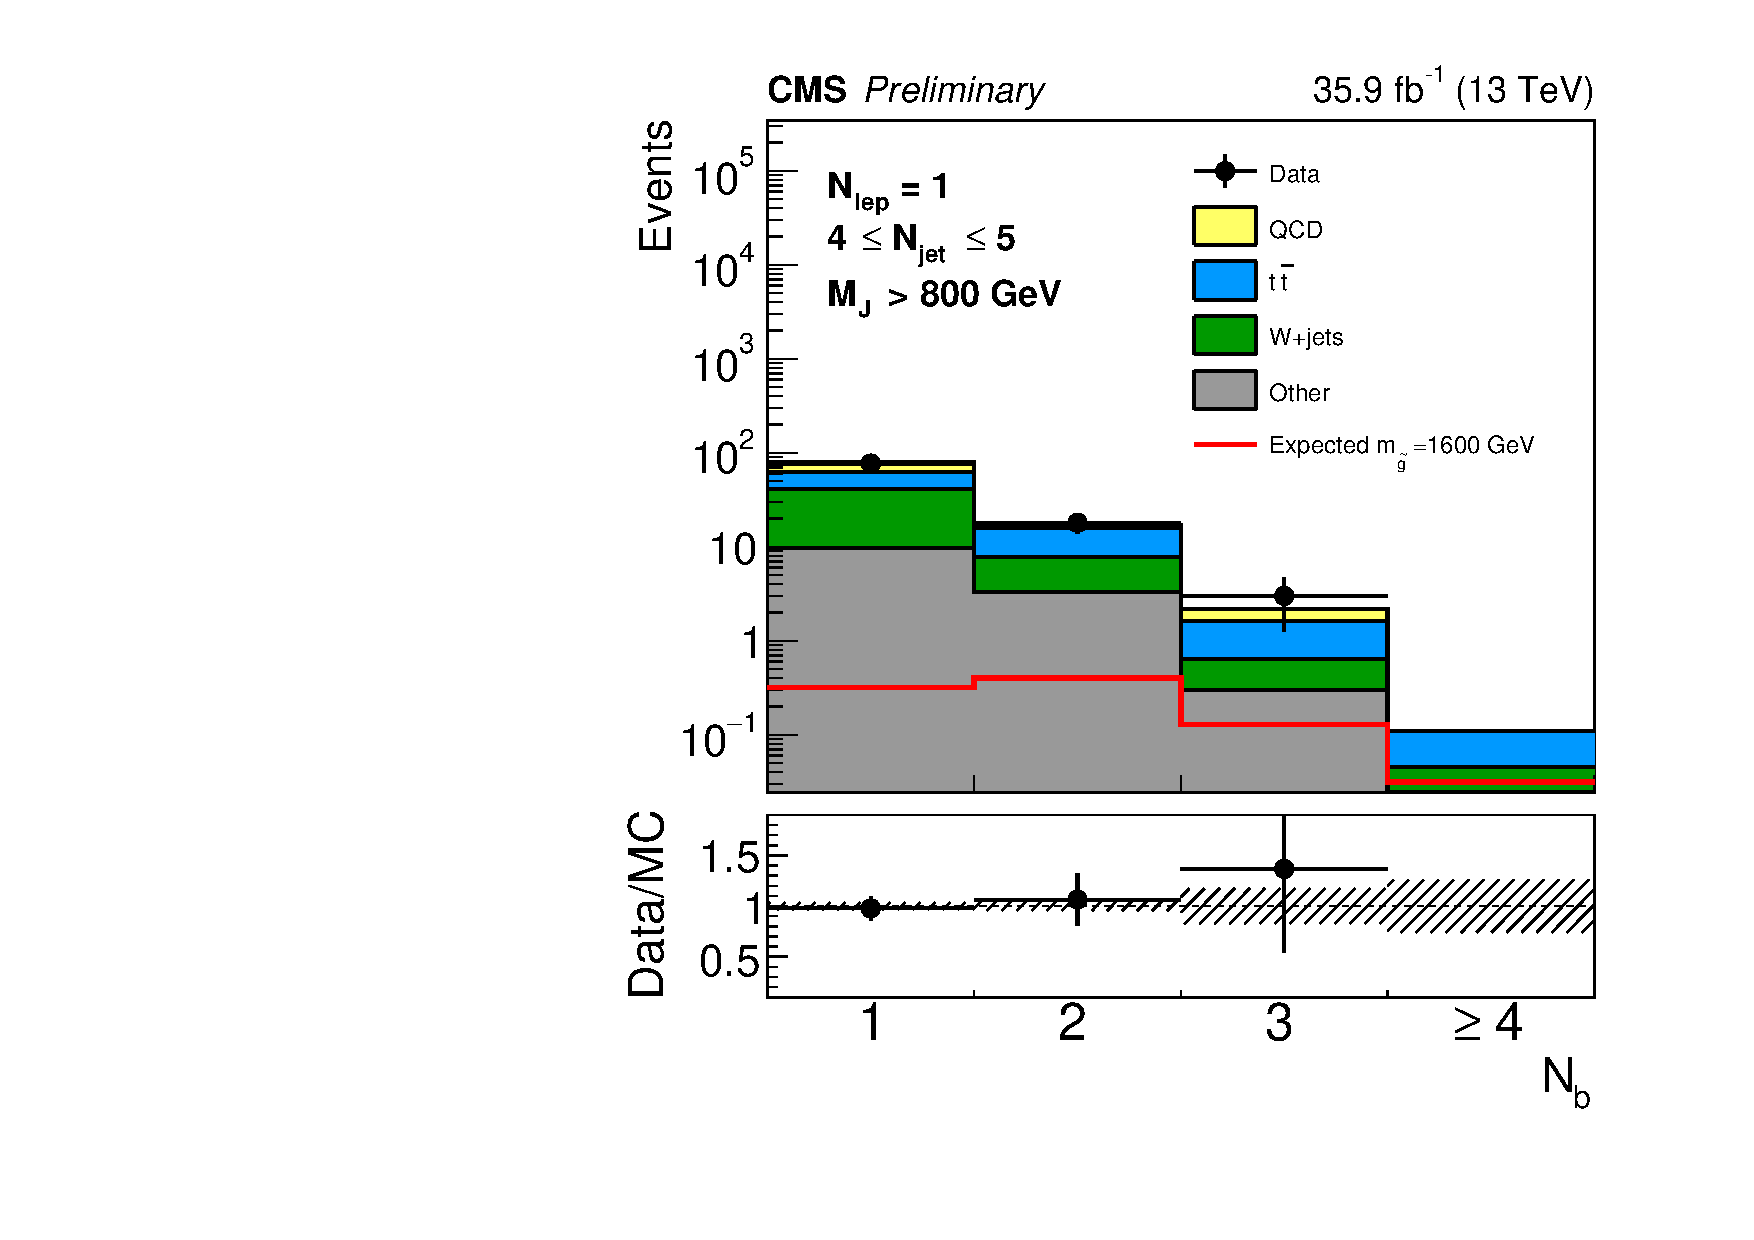
\includegraphics[angle=0,width=0.32\columnwidth]{fig/prefit_nlep1_nj45_highmj.pdf}
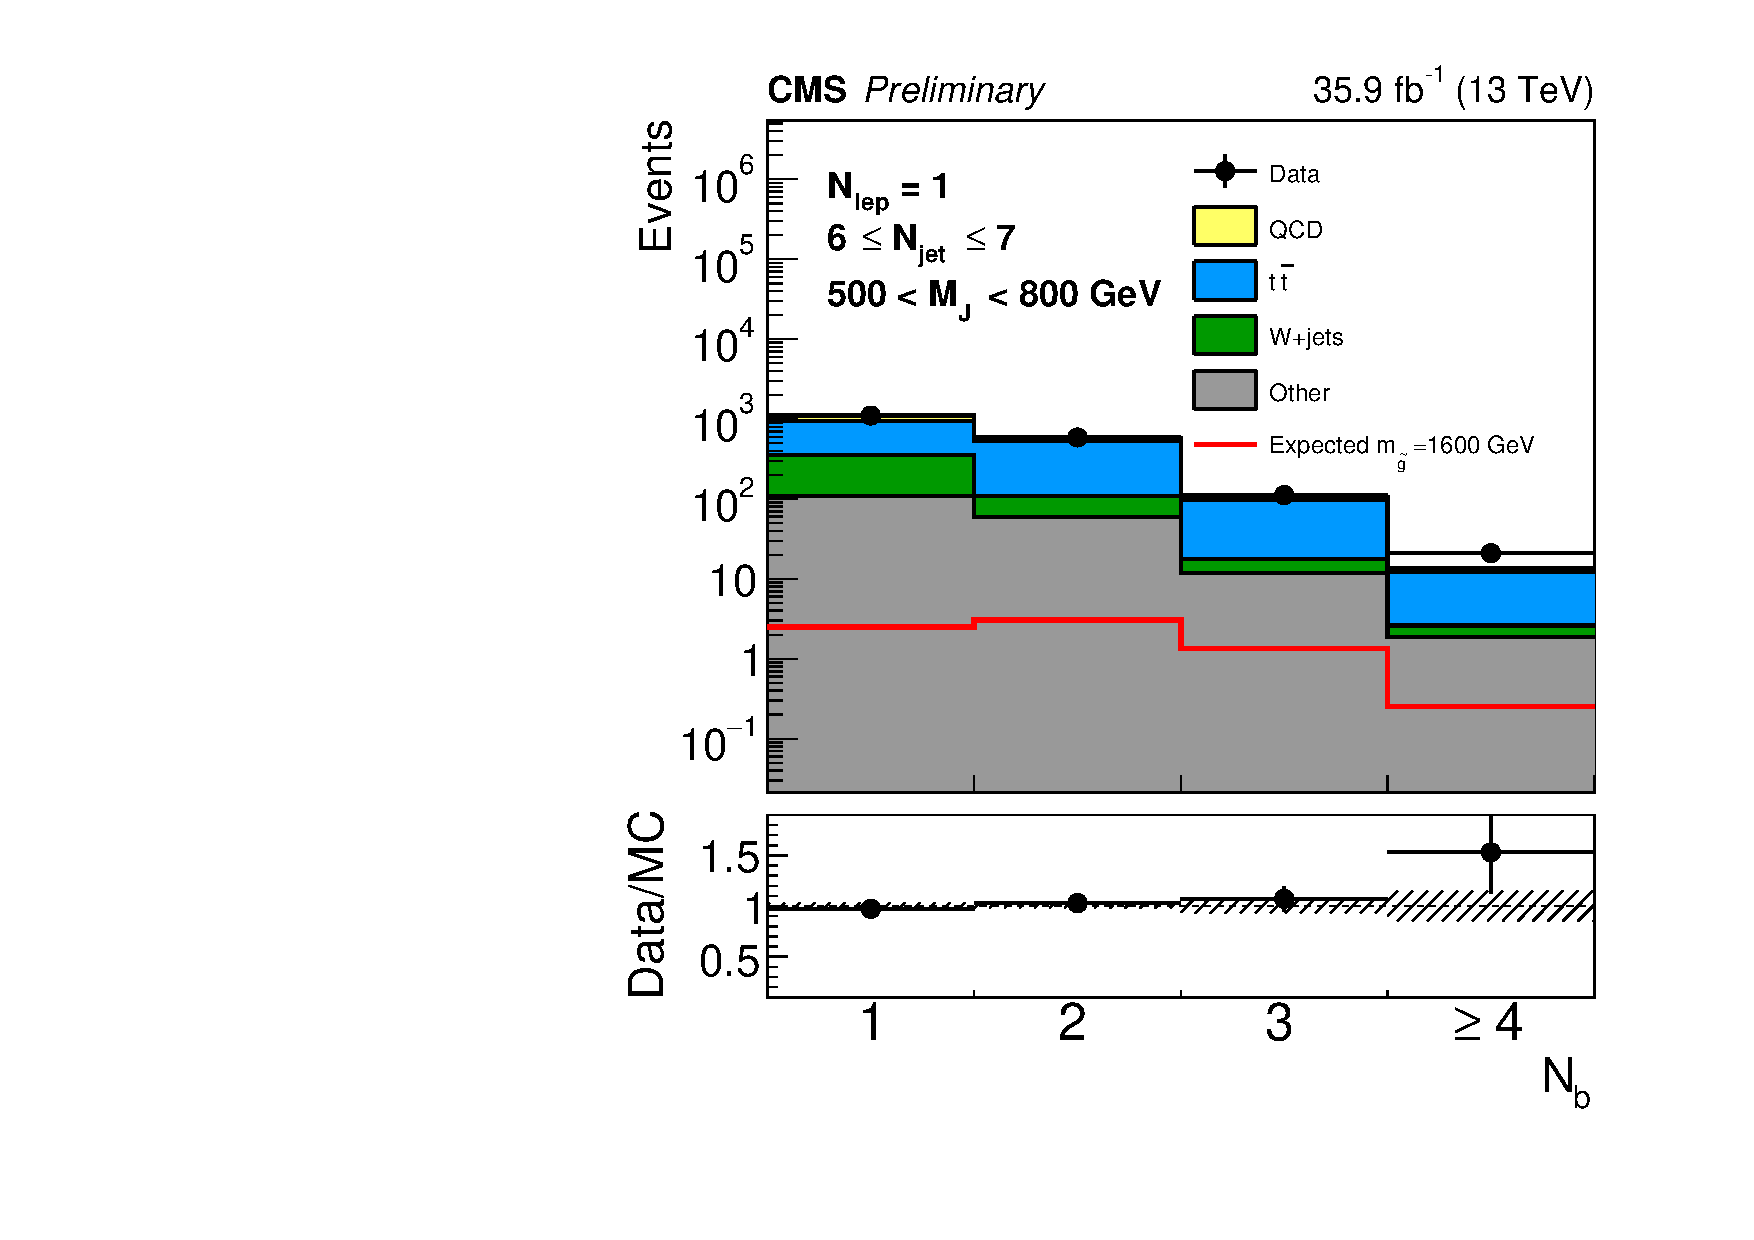
\includegraphics[angle=0,width=0.32\columnwidth]{fig/prefit_nlep1_nj67_lowmj.pdf}
\end{center}
\caption{Pre-fit \Nb distributions of the control region bins with the background simulation normalized to the observed data yields with a single scaling factor.
The ratio of data-to-simulation is shown in the lower panel.
The pre-fit uncertainty is represented by the hatched band.}
\label{fig:prefit_cr}
\end{figure}

Lastly, Table~\ref{tab:crfit_pulls} compares the post-fit pulls of the background-only and signal-plus-background control region fit.
The post-fit pulls between the two fits are fully consistent with each other, as is expected for these signal-poor regions.

\begin{table}[tbp!]
\begin{center}
\begin{tabular}{|l|c|c|c|} \hline
                                                  &  Post-fit pull     &  Post-fit pull     &                           \\
Nuisance parameter                                &  ($b$-only fit)    &  ($s+b$ fit)       &  $\rho(\theta_{m}, \mu)$  \\  
\hline
b,c jet b-tag SF (btag\_bc)                       &  $+0.13 \pm 0.98$  &  $+0.07 \pm 1.05$  &  -0.18                    \\
u,d,s,g jet b-tag SF (btag\_udsg)                 &  $+0.37 \pm 0.92$  &  $+0.28 \pm 0.95$  &  -0.26                    \\
Gluon splitting (gs)                              &  $+0.42 \pm 0.87$  &  $+0.22 \pm 1.12$  &  -0.43                    \\
Jet energy resolution (jer)                       &  $-0.02 \pm 0.63$  &  $-0.02 \pm 0.60$  &  -0.01                    \\
Jet energy scale (jes)                            &  $+0.03 \pm 0.63$  &  $+0.03 \pm 0.61$  &  -0.03                    \\
Lepton efficiency (lep\_eff)                      &  $-0.01 \pm 0.99$  &  $-0.01 \pm 0.99$  &  +0.01                    \\   
Luminosity (lumi)                                 &  $+0.00 \pm 0.99$  &  $+0.00 \pm 0.99$  &  -0.01                    \\   
Fact. scale for Other (other\_muf)                &  $-0.00 \pm 0.99$  &  $-0.00 \pm 0.99$  &  +0.00                    \\   
Renorm. scale for Other (other\_mur)              &  $-0.07 \pm 0.96$  &  $-0.06 \pm 1.02$  &  +0.02                    \\   
Renorm. and Fact. scale for Other (other\_murf)   &  $-0.06 \pm 0.98$  &  $-0.08 \pm 0.96$  &  +0.01                    \\   
QCD fake rate (qcd\_fakerate)                     &  $+0.05 \pm 1.01$  &  $+0.09 \pm 1.14$  &  +0.09                    \\   
Fact. scale for QCD (qcd\_muf)                    &  $-0.01 \pm 1.01$  &  $-0.01 \pm 1.01$  &  -0.00                    \\   
Renorm. scale for QCD (qcd\_mur)                  &  $+0.00 \pm 0.99$  &  $+0.00 \pm 0.99$  &  -0.00                    \\   
Renorm. and Fact. scale for QCD (qcd\_murf)       &  $-0.01 \pm 1.01$  &  $-0.01 \pm 1.01$  &  -0.00                    \\   
Fact. scale for \ttbar (ttbar\_muf)               &  $-0.01 \pm 1.01$  &  $-0.01 \pm 1.00$  &  +0.00                    \\   
Renorm. scale for \ttbar (ttbar\_mur)             &  $-0.00 \pm 1.00$  &  $+0.00 \pm 0.99$  &  +0.01                    \\   
Renorm. and Fact. scale for \ttbar (ttbar\_murf)  &  $-0.01 \pm 1.01$  &  $-0.01 \pm 1.00$  &  +0.01                    \\   
Fact. scale for \Wjets (wjets\_muf)               &  $-0.00 \pm 0.99$  &  $+0.00 \pm 0.99$  &  +0.00                    \\   
Renorm. scale for \Wjets (wjets\_mur)             &  $-0.00 \pm 0.99$  &  $-0.00 \pm 0.99$  &  -0.00                    \\   
Renorm. and Fact. scale for \Wjets (wjets\_murf)  &  $-0.00 \pm 1.00$  &  $-0.00 \pm 1.00$  &  +0.00                    \\   
\hline
\end{tabular}
\caption{Table of post-fit pulls of the background-only and signal-plus-background control region fit.
The last column, $\rho(\theta_{m}, \mu)$, lists the correlation between the corresponding nuisance parameter, $\theta_{m}$, and the nuisance parameter controlling the signal strength, $\mu$.}
\label{tab:crfit_pulls}
\end{center}
\end{table}

\end{subsection}
